%%%%%%%%%%%%%%%%%%%%%%%%%%%%%%%%%%%%%%%%%%%%%%%%%%%%%%%%%%%%%%%%%%%%%%%%%%%%
% AGUJournalTemplate.tex: this template file is for articles formatted with LaTeX
%
% This file includes commands and instructions
% given in the order necessary to produce a final output that will
% satisfy AGU requirements, including customized APA reference formatting.
%
% You may copy this file and give it your
% article name, and enter your text.
%
%
% Step 1: Set the \documentclass
%
%

%% To submit your paper:

%\RequirePackage{hyperref}
\documentclass[sn-mathphys,Numbered]{sn-jnl}
%\usepackage{url} %this package should fix any errors with URLs in refs.
%\usepackage{lineno}
%\usepackage[inline]{trackchanges} %for better track changes. finalnew option will compile document with changes incorporated.
%\usepackage{soul}
%\linenumbers
%%%%%%%
% As of 2018 we recommend use of the TrackChanges package to mark revisions.
% The trackchanges package adds five new LaTeX commands:
%
%  \note[editor]{The note}
%  \annote[editor]{Text to annotate}{The note}
%  \add[editor]{Text to add}
%  \remove[editor]{Text to remove}
%  \change[editor]{Text to remove}{Text to add}
%
% complete documentation is here: http://trackchanges.sourceforge.net/
%%%%%%%
\usepackage{url}
\usepackage{graphicx}%
\usepackage{multirow}%
\usepackage{amsmath,amssymb,amsfonts}%
\usepackage{amsthm}%
\usepackage{mathrsfs}%
\usepackage{stmaryrd}
\usepackage[title]{appendix}%
\usepackage{xcolor}%
%\usepackage{textcomp}%
\usepackage{manyfoot}%
\usepackage{booktabs}%
%\usepackage{algorithm}%
%\usepackage{algorithmicx}%
%\usepackage{algpseudocode}%
%\usepackage{listings}%

%


\newtheorem{theorem}{Theorem}
\newtheorem{prop}{Proposition}[theorem]

\def\Laplace{\Delta}
\def\prtl{\partial} % partial deriv.
\def\grad{\nabla}
\def\vc#1{\mathbf{\boldsymbol{#1}}}     % vector
\def\todo#1{{TODO:\color{red}#1}}
\def\ol#1{\overline{#1}}
\def\log{{\rm log}}
\def\abs#1{{|#1|}}


\begin{document}

%% ------------------------------------------------------------------------ %%
%  Title
%
% (A title should be specific, informative, and brief. Use
% abbreviations only if they are defined in the abstract. Titles that
% start with general keywords then specific terms are optimized in
% searches)
%
%% ------------------------------------------------------------------------ %%

% Example: \title{This is a test title}

\title[Article Title]{Analytical solution to a Darcy flow on a bounded fracture-matrix domain}
%% ------------------------------------------------------------------------ %%
%
%  AUTHORS AND AFFILIATIONS
%
%% ------------------------------------------------------------------------ %%

% Authors are individuals who have significantly contributed to the
% research and preparation of the article. Group authors are allowed, if
% each author in the group is separately identified in an appendix.)

% List authors by first name or initial followed by last name and
% separated by commas. Use \affil{} to number affiliations, and
% \thanks{} for author notes.
% Additional author notes should be indicated with \thanks{} (for
% example, for current addresses).

% Example: \authors{A. B. Author\affil{1}\thanks{Current address, Antartica}, B. C. Author\affil{2,3}, and D. E.
% Author\affil{3,4}\thanks{Also funded by Monsanto.}}

\author*[1]{\fnm{Jan} \sur{Brezina}}\email{jan.brezina@tul.cz}

\author[2]{\fnm{Pavel} \sur{Burda}}\email{pavel.burda@fs.cvut.cz}
\equalcont{These authors contributed equally to this work.}


\affil*[1]{\orgname{Technical University of Liberec}, \orgaddress{\city{Liberec}, \country{Czech Republic}}}
\affil[2]{\orgname{Czech Technical University}, \orgaddress{\city{Prague}, \country{Czech Republic}}}



\abstract{
We derive an analytical solution in terms of Fourier method to the Darcy flow problem
that combines a discrete fracture with a continuum matrix using the Fourier method. 
Separate equations for the fracture and matrix domain are considered, coupled by a Robin-type condition.

We investigate two cases: the continuous matrix pressure for a conductive fracture, and the discontinuous matrix pressure for a barrier fracture. To validate our solution, we compare it against a numerical solution using second-order finite differences in a parametric study. We also deal with efficient summation of the resulting series. Our results demonstrate the accuracy and effectiveness of the analytical solution, which is a valuable tool for testing new numerical schemes to the models with discrete fractures.
}

\keywords{analytical solution, discrete fracture-matrix, Darcy flow, Fourier method}




\maketitle
\section{Introduction}
Fractures ranging from cracks to faults are ubiquitous in crystalline rocks and have a significant impact on groundwater flow, despite occupying only a small fraction of rock volume. Open fractures with substantially higher permeability form preferential paths, leading to shorter breakthrough times in the transport of contaminants, while the healed fractures can behave as barriers.

Fractures occur on a wide range of scales. The effect of small-scale fractures can be homogenized and described by anisotropic and heterogeneous continuum \cite{Bogdanov2007Effective}. The large-scale fractures should rather be described explicitly in order to capture preferential paths
as in the DFN methods, e.g. \cite{Elmo_Discrete_2014a}. 
To capture both small- and large-scale fractures and their interactions, the {\emph discreate fracture-matrix} (DFM)  approach can be applied, where the continuum, 3D or 2D, is coupled with the fractures as objects of lower dimension, 2D or 1D, respectively. This approach was pioneered
by \cite{Martin2005} for the Darcy flow and later extended by a number of theoretical and numerical results \cite{Angot2009a}, \cite{fumagalli_numerical_2011}, \cite{brezina_analysis_2015}.  


To verify the accuracy of various numerical schemes for the DFM approach, it is important to use suitable test problems with known analytical solutions. While plugging in any function to the equations and prescribing the resulting right-hand side is a common approach, it may not capture the complexities of the real solution and may not be suitable for testing convergence of the numerical method. 

This work provides an analytical solution to the Darcy flow problem on a square domain (matrix) and a single horizontal fracture. Two cases are considered: the {\it conductive fracture} and the more general {\it barrier fracture}.
The conductive fracture case assumes symmetry about the fracture yet keeping separate pressure for the matrix and for the fracture. 
This case is relatively simple to solve but has very limited practical usage.
The barrier fracture case is a generalization where the problem parameters, as well as the matrix pressure, are treated independently on the upper and the lower part of the matrix domain. 
The analytical solutions to these problems are derived using the Fourier method for boundary value problems (see \cite{Brown1993}).
This work provides an analytical solution to the Darcy flow problem on a square domain (matrix) and a single horizontal fracture. Two cases are considered: the {\it conductive fracture} case and the {\it barrier fracture} case. The conductive fracture case assumes symmetry about the fracture while maintaining separate pressure for the matrix and the fracture, making it relatively simple to solve but with limited practical usage. On the other hand, the barrier fracture case is a generalization where the problem parameters and matrix pressure are treated independently on the upper and lower parts of the matrix domain, making it a more complex problem. The analytical solutions to both cases are obtained using the Fourier method for boundary value problems (see \cite{Brown1993}).


Excesive list of analytical solutions to various 1d advection-diffusion problems is derived in \cite{Genuchten1982}
 
 Both problems are introduced in Section \ref{sec:setting}.
The solution to the conductive fracture problem is derived in Section \ref{sec:continuous_frac}
using the Fourier method (see \cite{Brown1993} and \cite{Onder1998})

the same approach with necessary modifications and extensions
is used to derive the solution to the barrier fracture problem in Section \ref{sec:barrier_frac}. In Section \ref{sec:verify}, 
both solutions are verified against a numerical solution provided by the second-order finite difference scheme on a regular grid. 
Conclusions are summarized in the final Section \ref{sec:conclusion} 


Book about Fourier method:
\cite{Brown1993}

Application of the Fourier method to the Darcy flow problems: \cite{Onder1998}


\section{Problem formulation}
\label{sec:setting}
In this section, we present the Darcy flow problem for a discrete fracture-matrix system, considering two cases: the barrier fracture and the conductive fracture. The problem geometry, depicted in Figure \ref{fig:domains}, consists of a horizontal fracture $\Omega_1$ that splits a square domain (matrix) into upper and lower parts, $\Omega_2^+$ and $\Omega_2^-$, respectively.  The stationary Darcy flow on these domains is described by the equations:
\begin{align}
  \label{eq:Darcy_common}
  -k_1\, \partial_x^2 p_1(x) &= f(x) \qquad &&\text{ in }\Omega_1,\\
  -k_2^\pm\, \Laplace p^\pm_2(x,y) &= 0 \qquad &&\text{ in }\Omega_2^\pm.
  \label{eq:Darcy_common_c}
\end{align}
Here $p_1$, $p_2^{\pm}$ denote the pressure in corresponding domains and $f$ is the communication term that will be specified later. 
We assume the strictly positive conductivities $k_1$, $k_2^\pm$  on $\Omega_1$ and $\Omega_2^\pm$, respectively.

The no-flow boundary condition is imposed on the sides of $\Omega_2^\pm$:
\begin{equation}
  \prtl_x p_2(x,y) = 0  \quad\text{ on } \Gamma_2^N.    
  \label{eq:bc_neumann}
\end{equation}

The Dirichlet boundary condition is applied on the both tips of the fracture and on the top and bottom of the matrix domain, see Fig. \ref{fig:domains}:
\begin{align}
  \label{eq:bc_dirichlet_1}
  p_1(x) &= P_1          &&\text{ on } \Gamma_1,\\
  \label{eq:bc_dirichlet_2}
  p_2^\pm(x,y) &= P_2^\pm        &&\text{ on } \Gamma_2^\pm.
\end{align}


\begin{figure}
    \begin{center}
    \includegraphics[width=0.6\textwidth]{figs/domains.pdf}
    \caption{Notation of the domains and boundaries.}
    \label{fig:domains}
    \end{center}
\end{figure}

{\bf Barrier fracture.} 
To complete the problem formulation, we need to specify the coupling between the fracture and the matrix. This is done in terms of a Robin boundary condition for the matrix domain and a corresponding source term in the fracture. The Robin condition reads:
\begin{equation}
\label{eq:barrier_robin}
- k_2^\pm\, \grad p_2^\pm\cdot \vc n^\pm(x,0) 
  = f^\pm(x) =\sigma^\pm (p^\pm_2(x,0) - p_1(x)).
\end{equation}
where $\sigma^\pm \ge 0$ is a coupling parameter typically  proportional to $k_1$. 
The source term in $\Omega_1$ is then given by the sum of both boundary fluxes:
\begin{equation}
\label{eq:barrier_source}
f(x) = f^+(x) + f^-(x) \quad \text{ for }x\in\Omega_1.
\end{equation}


{\bf Conductive fracture.} For simplicity, we consider a vertically symmetric version of the problem. That implies symmetry of the matrix parameters $k_2 = k_2^\pm$, $P_2 =P_2^\pm$,  $\sigma = \sigma^\pm$, and continuity of the matrix pressure $p_2(x, 0) = p_2^\pm(x, 0)$ on $\Omega_1$. For $\sigma \ge k_1 \ge k_2$, this case can be interpreted as a conductive fracture, hence the name. Smaller values of $\sigma$ admit a physical interpretation of the fracture as  a fault zone formed by a network of small channels with less permeable walls.

The essential steps of the solution for the conductive fracture case of are described in Section \ref{sec:continuous_frac}, while the more technical  barrier fracture case is covered later in Section \ref{sec:barrier_frac}. 

\section{Conductive fracture}
\label{sec:continuous_frac}
To solve the conductive fracture problem, we will employ the classical Fourier method, see e.g. \cite{Brown1993}. 
First, we reduce the problem due to symmetries and formulate the main result about its analytical solution (Section \ref{sec:main_result_cf}). We then proceed to the solution for the matrix domain using the separation of variables technique (Section \ref{sec:p2_conductive}), followed by the solution for the fracture domain (Section \ref{sec:p1_conductive}), taking into account the influence of the matrix-domain solution. Both solutions have the form of cosine series with interrelated coefficients. These are determined in the final step (Section \ref{sec:cont_coupling}), where we plug the solutions into the Robin boundary condition that conveys the fracture's influence on the matrix. Finally, in Section \ref{sec:eval}, we summarize the evaluation procedure for the analytical solution and provide a basic convergence analysis of the involved series.


\subsection{Strong solution result}
\label{sec:main_result_cf}
The symmetry of the conductive fracture problem in both the $x$ and $y$ directions allows us to solve the system $(\ref{eq:Darcy_common} - \ref{eq:barrier_source})$ only in the first quadrant $\widetilde\Omega_2=(0,1)\times(0,1)$ and in the right half of the fracture $\widetilde\Omega_1=(0,1)$. The equivalent system of equations on the reduced domains is given by:
\begin{align}
    \label{eq:cc_darcy_2d}
    -k_1\, \partial_x p_1(x) &= f(x)               &&\text{on }\widetilde\Omega_1,\\
    -k_2\, \Laplace p_2(x,y) &= 0         &&\text{on }\widetilde\Omega_2,
    \label{eq:cc_darcy_1d}
\end{align}
accompanied by the boundary conditions for the fracture domain:\begin{equation}
    \label{eq:cc_bc_1}
    \partial_x p_1(0) = 0, \quad  p_1(1) = P_1, 
\end{equation}
and the following boundary conditions for the matrix domain:
\begin{align}
    \label{eq:cc_bc_x}
    p_2(x, 1) &= P_2, \quad
    \prtl_x p_2(0,y) = \prtl_x p_2(1,y) = 0,\\    
    \label{eq:cc_bc_robin}
    k_2\, \prtl_y p_2(x,0) &= \frac{f(x)}{2}
                        = \sigma(p_2(x,0) - p_1(x))
\end{align}
for $x, y\in (0,1)$.
%
%%%%%%%%%%%%%%%%%%%%%%%%%%%%%%%%%%%%%%%%%%% PROPOSITION 1
\newcommand{\kfrel}{\kappa_1}
\newcommand{\kmrel}{\kappa_2}
The existence and uniqueness of the weak solution to the reduced problem is a straight-forward excercise in application of the Lax-Milgram Lemma. In the following result, we however state existence of the strong solution in terms of cosine series.
\begin{theorem}
\label{proposition_continuous}
Let the pressures $P_2$, $P_1$ and possitive real parameters $k_1$, $k_2$, $\sigma$ be given. Then the unique strong solution $p_1(x)$ and $p_2(x,y)$ to the system 
$(\ref{eq:cc_darcy_2d} - \ref{eq:cc_bc_robin})$ can be expressed in form of cosine series:
\begin{align}
    \label{eq:p1_series}
    p_1(x) &= P_2 - b_0\big(1 + C \cosh(x/\kfrel)\big) -2b_0 \sum_{n=1}^\infty  u_n \cos(n \pi x),\\
    \label{eq:p2_series}
    p_2(x,y) &= P_2 - b_0(1-y) -2b_0 \sum_{n=1}^\infty b_n \cos(n \pi x) {\rm sinh} \big(n \pi(1-y)\big),
\end{align}
with coefficients:
\begin{align}
    \label{eq:un}
    u_n &= \frac{b_n \sinh(n \pi)}{1 + (\kfrel n \pi)^2},\\
    \label{eq:an}
    b_n &= \frac{(-1)^n}{n \pi \cosh(n \pi) \big(1 + (\kfrel n \pi)^2\big) 
    +  (n \pi \kfrel / \kmrel)^2 \sinh(n\pi)}.
\end{align}
and other parameters:

\begin{equation}
    \label{eq:u0}
    \kfrel = \sqrt{\frac{k_1}{2\sigma}}, \quad     
    \kmrel = \sqrt{\frac{k_2}{\sigma}}, \quad
    C =  \frac{\kmrel^2 }{\kfrel\sinh(1/\kfrel)},
\end{equation}

\begin{equation}
     \label{eq:b0}
     U =  \sum_{n=1}^{\infty} (-1)^n u_n, \quad
     b_0 = \frac{P_2 - P_1}{1 + 2  U + C\cosh(1/\kfrel)} 
\end{equation}

\end{theorem}


\subsection{\bf Separation of variables for 2D equation}
\label{sec:p2_conductive}
%
To find the solution in the matrix domain, we employ the separation of variables  (see e.g. \cite{Evans1998}) to the equation \eqref{eq:cc_darcy_2d}.  
We consider the solution in form $p_2(x,y) = X(x)Y(y)$ 
and substitute into \eqref{eq:cc_darcy_2d} to obtain the equations:
\[
\frac{X''}{X} = -\frac{Y''}{Y} = L.
\]  
Taking into account the homogeneous Neumann boundary conditions given in \eqref{eq:cc_bc_x}, we get possible solutions for $X(x)$ in the form:
\begin{equation}
    \label{eq:general_x}
    X_0(x) = 1, \quad X_n(x) = \cos (n\pi x)\qquad \text{ for }n=0,1, \dots,
\end{equation}
where the constant $L$ can only attain the discrete values:
\[
    L_n= - n^2 \pi^2.
\]
Now, we substitute $L_n$ into the linear equation for $Y(y)$. We write down its solution as function of $(1-y)$ in order to get simpler expressions for the Dirichlet condition later on:
\begin{align}
Y_0(y) &= A_0 + B_0 (1-y), \nonumber \\
\label{eq:general_y}
Y_n(y) &= A_n e^{n\pi (1-y)}+ B_n e^{-n\pi (1-y)}\qquad \text{ for } n =1, \dots.
\end{align}
where $A_n, B_n$ are arbitrary real numbers.
%
By combining \eqref{eq:general_x} and \eqref{eq:general_y}, we obtain the solution $p_2$ in form of series:
\begin{equation}
    \label{eq:p2_1}
    p_2(x, y) = A_0 + B_0 (1-y) + \sum ^{\infty}_{n=1} \cos (n\pi x) 
            \big(A_n e^{n\pi (1-y)} + B_n e^{-n\pi (1-y)}\big).
\end{equation}
We further constrain the coeficients by application of the  Dirichlet boundary condition from $(\ref{eq:cc_bc_x})$:
\[
    P_2 = A_0  + \sum ^{\infty}_{n=1} \cos (n\pi x) 
            \big(A_n  + B_n\big)\quad \text{for all }x\in (0, 1).
\]
As the functions $f_0=1$, $f_n =\cos(n\pi x)$ are linearly independent, we get equations for the coefficients by comparison to the left hand side: 
\[
    A_0  = P_2, \quad\text{ and } \quad A_n+B_n = 0.
\]
Using these relations, we can simplify the solution \eqref{eq:p2_1} to the final form \eqref{eq:p2_series} by setting $B_0= -b_0$ and $A_n=-B_n = -b_nb_0$.


\subsection{Pressure on fracture}
\label{sec:p1_conductive}

 Next step is solution of the equation \eqref{eq:cc_darcy_1d} in the reduced fracture domain $\tilde \Omega$. 
 Substituting for $f$ from right hand side of $(\ref{eq:cc_bc_robin})$ and then applying expansion \eqref{eq:p2_series} for $p_2(x, 0)$, 
 we arrive at the linear ODE: 
\begin{equation}
    \label{eq:p1_equation}
    -\kfrel^2 p_1''(x) + p_1 (x) = P_2 - b_0 - 2 b_0 \sum ^{\infty}_{n=1} b_n \sinh(n\pi)\, \cos (n\pi x).
\end{equation}
One can directly verify, that 
\[
    P_n(x) = \frac{\cos(n \pi x)}{1+\kfrel^2n^2\pi^2}
\]
is a particular solution to the linear ODE:
\[
    - \kfrel^2 P_n''(x) + P_n(x) = \cos(n \pi x).
\]
The characteristic equation provides roots $\lambda^\pm = \pm 1/\kfrel$
and appropriate exponential solution to the homogenous part. Summing the
homogeneous solution and linear combination of the particular solutions, we get the solution of \eqref{eq:p1_equation} in form:
\begin {equation}
    \label{eq:p1_general_sol}        
    p_1(x) = \frac{1}{2}\big(c^+ e^{x/\kfrel} + c^- e^{-x/\kfrel}\big) + P_2 - b_0 
    - 2 b_0 \sum^{\infty}_{n=1} u_n \cos (n\pi x).
\end {equation}
with $u_n$ given by \eqref{eq:un}. Then the Dirichlet and Neumann boundary conditions \eqref{eq:cc_bc_1} determine $c^\pm$ 
through the linear system:
\begin{align}
\label{eq:P1_dirichlet}
P_1 &= p_1(1) = \frac{1}{2}\big(c^+e^{1/\kfrel} + c^- e^{-1/\kfrel}\big) + P_2 - b_0 - 2 b_0 U, \\
0 &= p_1'(0) = \frac{1}{2\kfrel}(c^+ - c^-) 
\end{align}
with $U$ given by \eqref{eq:b0}. Using the second equation and 
plugging $c^\pm=-b_0C$ into \eqref{eq:p1_general_sol}, 
we obtain the pressure on fracture \eqref{eq:p1_series}.
Then the first equation \eqref{eq:P1_dirichlet} yeilds
the expression  \eqref{eq:b0} for $b_0$ while the parameter 
$C$ has yet to be determined.



\subsection{Fracture coupling}
\label{sec:cont_coupling}

Last relation that we have to exploit is the Robin boundary condition in $(\ref{eq:cc_bc_robin})$. We substitute already dicovered series \eqref{eq:p1_series} and \eqref{eq:p2_series} for $p_1$ and $p_2$, respectively, and we divide by $b_0$. Then collecting the coefficients of the Fourier series on the left-hand side and remaining function of $x$ on the right-hand side, we arrive at:
%  \[
%      b_0 \kmrel^2     % \prtl_y p_2 
%      + 2 b_0 \sum_{n=1}^\infty \Big[  
%          \kmrel^2 n\pi  \cosh(n \pi) % \prtl_y p_2 
%          + \sinh(n \pi) % -p_2
%          - \frac{\sinh(n \pi)}{1 + (\kfrel n \pi)^2} 
%      \Big] b_n \cos(n \pi x)        
%      = b_0 C \cosh(x/\kfrel) 
%  \]
\begin{equation}
    \label{eq:conductive_fourier_coupling}
    \frac{{\cal A}_0}{2} + \sum^{\infty}_{n=1} {\cal A}_n \cos (n\pi x) =  C \cosh(x/\kfrel)
\end{equation}
with
\begin{equation}
    \label{eq:fourier_A0}
    {\cal A}_0 = 2 \kmrel^2,
\end{equation}
\begin{equation}
    \label{eq:fourier_An} 
        {\cal A}_n = 2 b_n \Bigl[ \kmrel^2 n\pi \cosh(n\pi) - \frac{\sinh(n \pi)}{1 + (\kfrel n \pi)^2}  
    + \sinh(n \pi) \Bigr]\quad \text{for $n=1, \dots$}
\end{equation}
%
In order to express the remaining unknowns $C$, $b_n$, $n=1,\dots$,
we compare the Fourier coefficeints ${\cal A}_n$ on the left-had side of \eqref{eq:conductive_fourier_coupling}  to the Fourier expansion of the right-hand side $g(x)=C\cosh(x/\kfrel)$ with the coefficients:
\[
   {\cal B}_0 = 2\int_0^1 g(x) dx, \quad {\cal B}_n = 2\int_0^1 g(x) cos(n \pi x) dx.
\]
%
From the comparison of the absolute terms:
\begin{equation}
    \label{eq:compute_A0}
    {\cal A}_0 = {\cal B}_0 = 2 C \int _0^1 \cosh(x/\kfrel) dx =
    2  C \kfrel\sinh(1/\kfrel),
\end{equation}
%
we get expression \eqref{eq:u0} for $C$.
%
%
To deal with ${\cal B}_n$, we integrate by parts:
\[
 I_n = \int _0^1 \cosh(x/\kfrel) \cos (n\pi x) dx 
    = \frac{(-1)^n \kfrel}{1+(\kfrel n \pi)^2}\sinh(1/\kfrel).
\]
Then, substitution for $C$ yields:
\begin{equation}
    \label{eq:compute_An}
    {\cal A}_n = {\cal B}_n = 2 C I_n =  2\frac{(-1)^n \kmrel^2}{1+(\kfrel n \pi)^2},
\end{equation}
and further simplification leads to formula \eqref{eq:an} for coefficients $b_n$.

\subsection{Evaluation procedure}
\label{sec:eval}
The formulas provided in Theorem \ref{proposition_continuous} are not suitable for practical calculations due to evaluation of the hypergeometric functions for large values of $n$. To address this issue, we can factor out and cancel the growing term $e^{n \pi}$. Actual evaluation of the solution then folow the procedure below:

\begin{enumerate}
    \item Set finite $N$ for truncated series. 
    \item Compute $\tilde b_n$ for $n = 1, \dots, N$ using the formula:
    \[
        \tilde b_n = \frac{(-1)^n}{n \pi (1 - e^{-2n \pi}) \big(1 + (\kfrel n \pi)^2\big) 
            + (\kfrel / \kmrel\, n \pi)^2 (1 + e^{-2n \pi})} \ , 
    \]
    \item Compute related $\tilde u_n$ coefficients:
    \[
        \tilde u_n = \frac{\tilde b_n (1 - e^{-2n \pi})}{1 + (\kfrel n \pi)^2}, 
    \]
    \item Approximate $U$ by trunacated series:
    \[
        U \approx  \sum_{n=1}^{N} (-1)^n \tilde u_n.
    \]
    \item Compute the remaining parameters $C$, $b_0$ using \eqref{eq:u0}, \eqref{eq:b0}.
    \item Evaluate $p_2$ for any given point $(x,y)$ in $\Omega_2$ using the modified formula \eqref{eq:p2_series}:
    \[
        p_2(x,y) = P_2 - b_0(1-y) -2b_0 \sum_{n=1}^N \tilde b_n \cos(n \pi x) 
        \Big( e^{-n \pi |y|} - e^{n \pi (|y|-2)}\Big).
    \]
    \item Evaluate $p_1$ for any given $x$ in $\Omega_1$ using unmodified formula \eqref{eq:p1_series}:
    \[
        p_1(x) = P_2 - b_0\big(1 + C\cosh(x/\kfrel)\big) - 2 b_0 \sum_{n=1}^N  u_n \cos(n \pi x). 
    \]    
\end{enumerate}

It is also important to consider the convergence rates of the series for practical usage.   
Series for $p_2$ converge exponentially for $y\ne 0$. 
For $\tilde b_n$ we have:
\[
    \tilde b_n \approx (-1)^n n^{-3} 
\]
and one order better decrease for two consecutive terms:
\[
    \abs{\tilde b_n + \tilde b_{n+1}} \approx n^{-3} - (n+1)^{-3} \approx  n^{-4}. 
\]
The truncation error for the series $n^{-k}$ can be bounded by integral: 
\[
    \sum_{i=N}^\infty n^{-k} \le O(N^{-(k-1)}).
\]
Therefore, on the line $y=0$, the the truncation error of the $p_2$ series is $O(N^{-3})$ at $x=0$, but close to $x=\pm 1$ the alternation of $\tilde b_n$ cancels out with the alterantion of $\cos(n \pi)$ and the error increases to $O(N^{-2})$.
Convergence of $u_n$ is better, namely:
\[
    \abs{u_n} \approx (-1)^n n^{-5},\qquad \abs{u_n+u_{n+1}} \approx  n^{-6}.
\]
Thus for the calculation of $p_1$, we have an error $O(N^{-5})$
for $x=0$, increasing to  $O(N^{-4})$ close to $x=\pm 1$. The error in $U$ approximation is $O(N^{-4})$ due to alternation canceled with $b_n$.
The practicaly observed behavior of errors follows these estimates. 



\section{Barrier fracture}
\label{sec:barrier_frac}
We use a similar approach to solve the case with a discontinuous $p_2$ across the fracture as for the continuous fracture case, but the procedure is slightly more technical. To make it more accessible, we begin with derivation of the solution, postponing formulation of the existence result. In Section \ref{sec:dom_sol}, we present the solutions in the individual domains, which closely follow the continuous fracture case.  The coupling of the domains ,described in Section \ref{sec:barrier_coupling}, leads to a sequence of 2x2 linear systems for the series coefficients. Finally, we formulate the existence result and summarize the evaluation procedure in Section
\ref{sec:barrier_result}.


\subsection{Domain solutions}
\label{sec:dom_sol}
Exploiting the $y$ axis symmetry of the problem $(\ref{eq:Darcy_common} - \ref{eq:barrier_source})$, we can consider the same system of equations 
on reduced domains $\Omega_2^+ = (0,1)\times (0,1)$, $\Omega_2^- = (0,1)\times(-1,0)$,
$\Omega_1 = (0,1)$. To impose the symmetry we consider homogeneous Neumann boundary condition on the $y$ axis $\{(0,y)\}$.
Repeating arguments from Section \ref{sec:p2_conductive} we obtain Fourier expansion for $p_2^+$ and $p_2^-$ similar to \eqref{eq:p2_series}:
\begin{align}
    \label{eq:p2_barrier_p}
    p_2^+(x,  y) &= P_2^+ + b_0^+(1-y) - D\sum_{n=1}^\infty b_n^+ \cos(n \pi x) {\rm sinh} \big(n \pi(1-y)\big),\\ 
    \label{eq:p2_barrier_m}
    p_2^-(x, -y) &= P_2^- + b_0^-(1-y) - D\sum_{n=1}^\infty b_n^- \cos(n \pi x) {\rm sinh} \big(n \pi(1-y)\big).
\end{align}
for any value of $D$ that will be specified later.
%
The equation for $p_1$ on $\Omega_1$ can be converted to the form similar to \eqref{eq:p1_equation}:
\begin{equation}
    \label{eq:p1_barrier_equation}
    - \ol{\kappa}_1^2  p_1''(x) + p_1(x) = \ol{P}_2 + \ol{b}_0 - D\sum_{n=1}^{\infty} \ol{a}_n \cos(n \pi x) \sinh(n \pi)
\end{equation}
where we have used averaged variables:

% \begin{align}
%     \label{eq:avg_sigma}
%     \ol{\sigma} &= (\sigma^+ + \sigma^-), \\
%     \label{eq:avg_k}
%     \ol{\kappa}_1 &= \sqrt{k_1/\ol{\sigma}},\\
%     \label{eq:avg_P2}
%     \ol{P}_2 &= \frac{\sigma^+ P_2^+ + \sigma^- P_2^-}{\ol{\sigma}}, \\
%     \label{eq:avg_B0}
%     \ol{b}_0 &= \frac{\sigma^+ b_0^+ + \sigma^- b_0^-}{\ol{\sigma}}, \\
%     \label{eq:avg_an}
%     \ol{A}_n &= \frac{\sigma^+ A_n^+ + \sigma^- A_n^-}{\ol{\sigma}}.  
% \end{align}

\begin{gather*}
    \ol{\sigma} = (\sigma^+ + \sigma^-), \qquad
    \ol{\kappa}_1 = \sqrt{k_1/\ol{\sigma}}, \qquad
    \ol{P}_2 = \frac{\sigma^+ P_2^+ + \sigma^- P_2^-}{\ol{\sigma}}, \\
%    
    \ol{b}_0 = \frac{\sigma^+ b_0^+ + \sigma^- b_0^-}{\ol{\sigma}}, \qquad
    \ol{b}_n = \frac{\sigma^+ b_n^+ + \sigma^- b_n^-}{\ol{\sigma}}.  
\end{gather*}

Then we can repeat steps from Section \ref{sec:p1_conductive} to get $p_1$ expansion that closely follows \eqref{eq:p1_series}:
\begin{equation}
    \label{eq:barrier_p1_series}
    p_1(x) = \ol{P}_2 +  \ol{b}_0 - D\cosh(x/\ol{\kappa}_1)\big) - D \sum_{n=1}^\infty  \ol{u}_n \cos(n \pi x) 
\end{equation}
with 
\begin{equation}
    \label{eq:barrier_un}
    \ol{u}_n = \frac{\ol{b}_n \sinh(n \pi)}{1 + (\ol{\kappa}_1 n \pi)^2}, \qquad
    \ol{U} =  \sum_{n=1}^{\infty} (-1)^n \ol{u}_n.
\end{equation}
Here we intentionaly set the free parameter $D$ to be equal to the integration constant \eqref{eq:p1_int_const}. The relation for the integration constant leads to:
\[
    \label{eq:barrier_D_eq}    
    \ol{P}_2 + \ol{b}_0 -D\cosh(1/\ol{\kappa}_1) - D \ol{U} = P_1,
\]
\begin{equation}
    \label{eq:barrier_D_expr}    
    D = \frac{\ol{P}_2- \ol{P}_1 + \ol{b}_0}{\ol{U} +\cosh(1/\ol{\kappa}_1)},
\end{equation}
where $\ol{b}_0$ given in terms of $b_0^{\pm}$ has yet to be determined.

\subsection{Coupling}
\label{sec:barrier_coupling}
As in Section \ref{sec:cont_coupling}, we plug expansion of $p_2^+$, $p_2^-$, and $p_1$ into \eqref{eq:barrier_robin}. 
We group the terms to get Fourier expansion on the left hand side and a known function of $x$ on the right hand side and we divide by $D$.
In particular, we have:
% \[
%   \frac{k_2^+ b_0^+}{\sigma^+} - P_2^+ + \ol{P}_2) + b_0^+ - \ol{b}_0
%   +\sum_{n=1}^{\infty} \Big[
%         2 \frac{k_2^+ b_0^+}{\sigma^+}  b_n^+ ( n \pi)  \cosh(n \pi) 
%        + 2b_0^+  b_n^+  \sinh(n \pi)   
%        -2\ol{b}_0 u_n   
%         \Big]
%         \cos(n \pi x)  
%   = 
%    - u_0 \cosh(x/\ol{\kappa}_1)
% \]
% 

\begin{equation}
    %\label{eq:fourier_coupling}
    \frac{{\cal A}_0^\pm}{2} + \sum^{\infty}_{n=1} {\cal A}_n^\pm \cos (n\pi x) = \cosh(x/ \ol{\kappa}_1).
\end{equation}
with
\begin{align}
    \label{eq:calA0_1}
    {\cal A}_0^\pm &= \frac{2}{D}\Big(-(\kappa_2^\pm)^2 b_0^\pm - P_2^\pm + \ol{P}_2 - b_0^\pm + \ol{b}_0\Big)\\
    \label{eq:calAn_1}
    {\cal A}_n^\pm          &=  
    b_n^\pm \Big( 
            n \pi (\kappa_2^\pm)^2  \cosh(n \pi) 
            +  \sinh(n \pi)  
           \Big) 
        - \ol{u}_n   
\end{align}
We reuse the calculation of Fourier coefficients of the right hand side from \eqref{eq:compute_A0} and \eqref{eq:compute_An} to obtain:
\begin{align}
    \label{eq:calA0_2}
    {\cal B}_0 &= 2 \ol{\kappa}_1 \sinh( 1/\ol{\kappa}_1 ), \\
    \label{eq:calAn_2}
    {\cal B}_n &=  2 \frac{(-1)^n    \ol{\kappa}_1}{1+(\ol{\kappa}_1 n \pi)^2}\sinh(1/\ol{\kappa}_1).
\end{align}
%
Now we combine \eqref{eq:calAn_1} and \eqref{eq:calAn_2}, and we substitute for $\ol{u}_n$ using \eqref{eq:barrier_un}.
We obtain a system to determine $b_n^+$, $b_n^-$:

\begin{equation}
    \label{eq:an_system}
    \begin{pmatrix} 
            X_n^+ & X_n \\ 
            X_n & X_n^-
    \end{pmatrix}
    \begin{pmatrix} 
        b_n^+  \\ 
        b_n^-     
    \end{pmatrix}
     =  
    \begin{pmatrix} 
        \sigma^+{\cal B}_n \\ 
        \sigma^-{\cal B}_n
    \end{pmatrix}
\end{equation}
where
% \[
% -\frac{2u_0 \ol{\kappa}_1}{1+(\ol{\kappa}_1 n \pi)^2}\sinh(1/\ol{\kappa}_1) = A_n^+ \Big( n \pi \frac{k_2^+ }{\sigma^+}  \cosh(n \pi) 
%         +     \sinh(n \pi)  \Big) 
%         - \frac{\sigma^+ A_n^+}{\ol{\sigma}}\frac{\sinh(n \pi)}{1 + (\ol{\kappa}_1 n \pi)^2}
%         - \frac{\sigma^- A_n^-}{\ol{\sigma}}\frac{\sinh(n \pi)}{1 + (\ol{\kappa}_1 n \pi)^2}
% \]
% 
% \[
% A_n^+ \Big( n \pi \frac{k_2^+ }{\sigma^+}  \cosh(n \pi) 
%         +     \sinh(n \pi)  - \frac{\sigma^+ }{\ol{\sigma}}\frac{\sinh(n \pi)}{1 + (\ol{\kappa}_1 n \pi)^2}\Big)     
%         - A_n^-\frac{\sigma^- }{\ol{\sigma}}\frac{\sinh(n \pi)}{1 + (\ol{\kappa}_1 n \pi)^2}
%         =
%         -\frac{2u_0 \ol{\kappa}_1}{1+(\ol{\kappa}_1 n \pi)^2}\sinh(1/\ol{\kappa}_1)
% \]

\begin{align}
    \label{eq:yn}    
    X_n^\pm  &= \sigma^\pm(n \pi \kappa_2^\pm\cosh(n \pi) 
              + \sinh(n \pi))  -  \frac{(\sigma^\pm)^2}{\ol\sigma} \ol{X}_n, \\    
    X_n  &= -\frac{\sigma^- \sigma^+}{\ol\sigma} \ol{X}_n, \\    
    \ol{X}_n &= \frac{\sinh(n \pi)}{1 + (\ol{\kappa}_1 n \pi)^2},
\end{align}
The system matrix is strictly diagonally dominant providing $k_2^{\pm}$, $\sigma^{\pm}$, $k_1$ are positive. Indeed comparing just the $\sinh$ terms, we have:
\[
 {\ol\sigma}\sigma^\pm (1 + (\ol{\kappa}_1 n \pi)^2)  - (\sigma^\pm)^2 
 > \sigma^- \sigma^+.
\]
%
Therefore the system has unique solution and the coefficients $b_n^{+/-}$ have the sign $(-1)^n$. This cancels out in the series \eqref{eq:barrier_un} for  $\ol{U}$ and makes $\ol{U}$ always positive.
%
Now, we compare \eqref{eq:calA0_2} to \eqref{eq:calA0_1}, we multiply by $D$ and substitute for it from  \eqref{eq:barrier_D_expr} to 
obtain a system for $b_0^+$, $b_0^-$:

\begin{equation}
    \label{eq:B0_system}
    \begin{pmatrix} 
            X^+_0 & \sigma^- X_0 \\ 
            \sigma^+ X_0 & X^-
    \end{pmatrix}
    \begin{pmatrix} 
        -b_0^+  \\ 
        -b_0^-     
    \end{pmatrix}
     =  
    \begin{pmatrix} 
        \sigma^+(P^+_2 - P_b) \\ 
        \sigma^-(P^-_2 - P_b)
    \end{pmatrix}
\end{equation}
where
\begin{align}
    %\label{eq:B0_system_p}
    P_b &= t \ol{P}_2 + (1-t) P_1, \\
    X_0^\pm &= (1+\kappa_2^\pm)  -t\frac{\sigma^+}{\ol{\sigma}}, \\
    X_0 &= -\frac{t}{\ol{\sigma}},\\
    t=1- \frac{\ol{\kappa}_1\sinh( 1/\ol{\kappa}_1 )}{\cosh(1/\ol{\kappa}_1) + \ol{U}}.
\end{align}
To show that the system matrix is non-singular, we first realise that:
\[
    0 < (1-t) \le \ol{\kappa}_1\, {\rm tanh}( 1/\ol{\kappa}_1 ) < 1,
\]
since $\ol{U}\ge0$, and we assue $\ol{\kappa}_1 > 0$. Next, we denote 
$a, b = (1+\kappa_2^\pm)$, and we estimate a determinant of the system 
\eqref{eq:B0_system}:
\[
  \Big(  a  -\frac{t}{\ol{\sigma}\sigma^+}\Big)
  \Big(b  -\frac{t}{\ol{\sigma}\sigma^-}\Big) - \frac{t^2}{\ol{
  \sigma^2}}\sigma^+\sigma- \ge ab - \frac{a\sigma^+ +b\sigma^-}{\sigma^+ +\sigma-} > 0,
\]
since $a, b > 1$. 


% Rovnice pro symetricka data:
% \[
%     \tilde b_0 = \frac{(P_2 - P_1)}{1 + \frac{\tilde U}{\sigma k \sinh(1/k)} + \frac{k_2\cosh(1/k)}{\sigma k \sinh(1/k)}   }
% \]
% 
% 
% 
% \[
%     [n \pi k_2 \cosh(n \pi) + \sigma\sinh(n \pi) ]A_n = - \frac{(-1)^n 2 \sigma k}{1+(k n \pi)^2}\sinh(1/k)
% \]
% 
% 
% \[
% [ n \pi k_2  \cosh(n \pi) + \sigma\sinh(n \pi) ] A_n = -\frac{(-1)^n 2 \sigma k}{1+(k n \pi)^2}\sinh(1/k)
% \]


\subsection{Strong solution result}
\label{sec:barrier_result}
Similary to the continuous fractue case, the existence and uniqueness of the weak solution to the system 
$(\ref{eq:Darcy_common} - \ref{eq:barrier_source})$ 
follows from the Lax-Milgram theorem. The above procedure demonstrates the existence of the unique strong solution  and enables us to state the folowing result:

\begin{theorem}
\label{proposition_continuous}
Given pressures $P_2^\pm$, $P_1$, and possitive real parameters $k_1$, $k_2^\pm$, $\sigma^\pm$, the system
$(\ref{eq:Darcy_common} - \ref{eq:barrier_source})$ 
has a unique strong solution that can be written in the form of cosine series \eqref{eq:p2_barrier_p} for $p_2^\pm(x, y)$, and \eqref{eq:barrier_p1_series} for $p_1(x)$. The coefficients of
the series are given by the sequence of regular linear systems \eqref{eq:an_system} and \eqref{eq:B0_system} for $b_n^\pm$ and $b_O^\pm$, respectively.
\end{theorem}

To practicaly evaluate $p_2(x,y)$ and $p_1(x)$, we use an approximation in terms of truncated
series. The coefficients $b_n^{\pm}$ are mutliplied by $e^{n\pi}$ as in Section \ref{sec:eval} to avoid overflow of floating-point arithemtic. The coefficients are determined through the following procedure:
\begin{enumerate}    
    \item
    Choose a finite length $N$ for the truncated series.
    \item 
    Solve the systems \eqref{eq:an_system} to obtain $b_n^\pm$,  for $n=1,\dots, N$.    
    \item 
    Compute $\ol{u}_n$ and the truncated sum $\ol{U}$ according to \eqref{eq:barrier_un}.
    \item 
    Solve the system \eqref{eq:B0_system} for $b_0^\pm$.    
    \item 
    Compute $D$ using \eqref{eq:barrier_D_expr}.
\end{enumerate}
The convergence properties of the series 
\eqref{eq:p2_barrier_p}, \eqref{eq:barrier_p1_series}, and \eqref{eq:barrier_un} are the same as those described in Section \ref{sec:eval}.







\section{Verification by finite differences}
\label{sec:verify}

\begin{figure}[h]
  
  \centering
  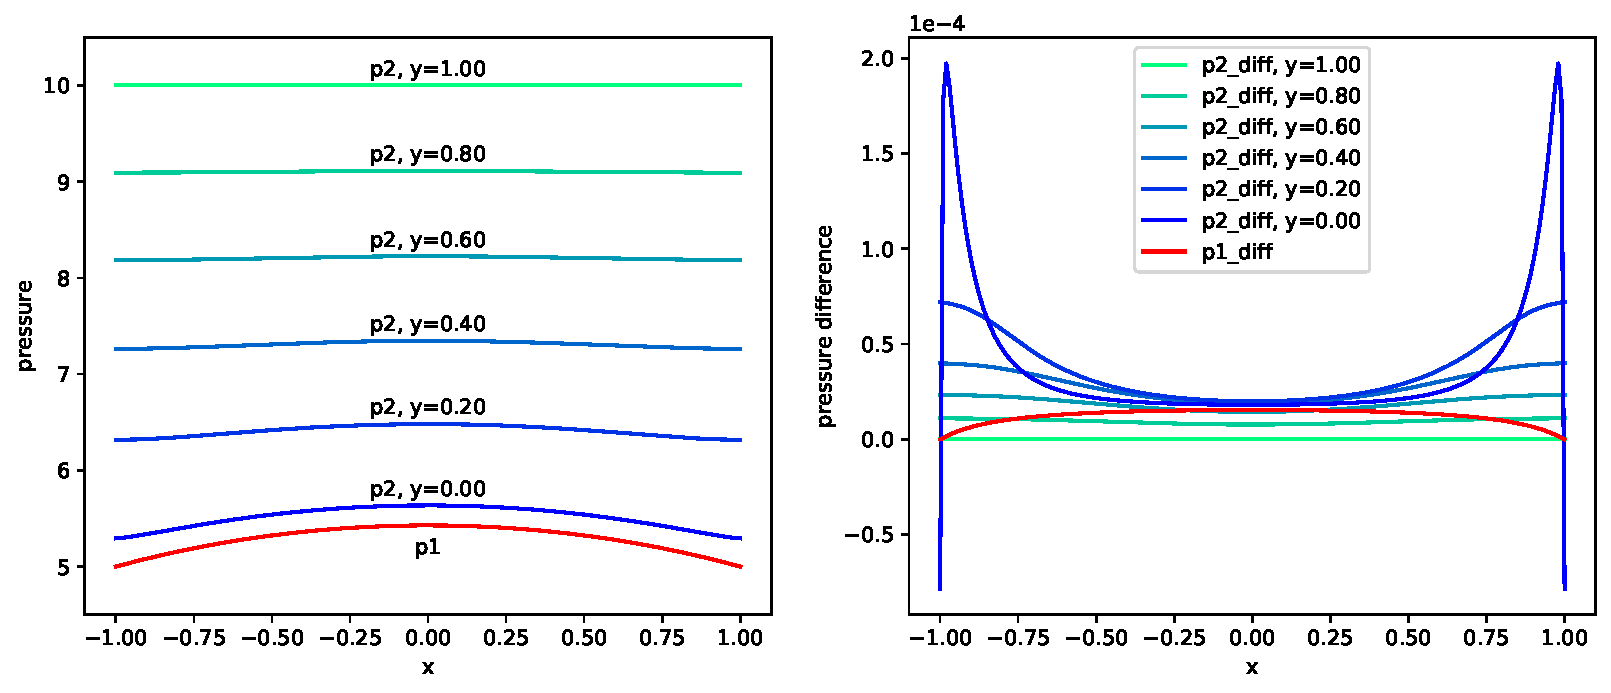
\includegraphics[width=\textwidth]{figs/continuous_solution.pdf}
  % continuous_convergency.pdf: 0x0 pixel, 300dpi, 0.00x0.00 cm, bb=
  \caption{Conductive fracture case. 
  {\it Left:} Match between the analytical and the numerical solution. 
  {\it Right:} Difference of the analytical and the numerical solution.}
  \label{fig:cont_solution}
\end{figure}



\begin{figure}
  
  \centering
  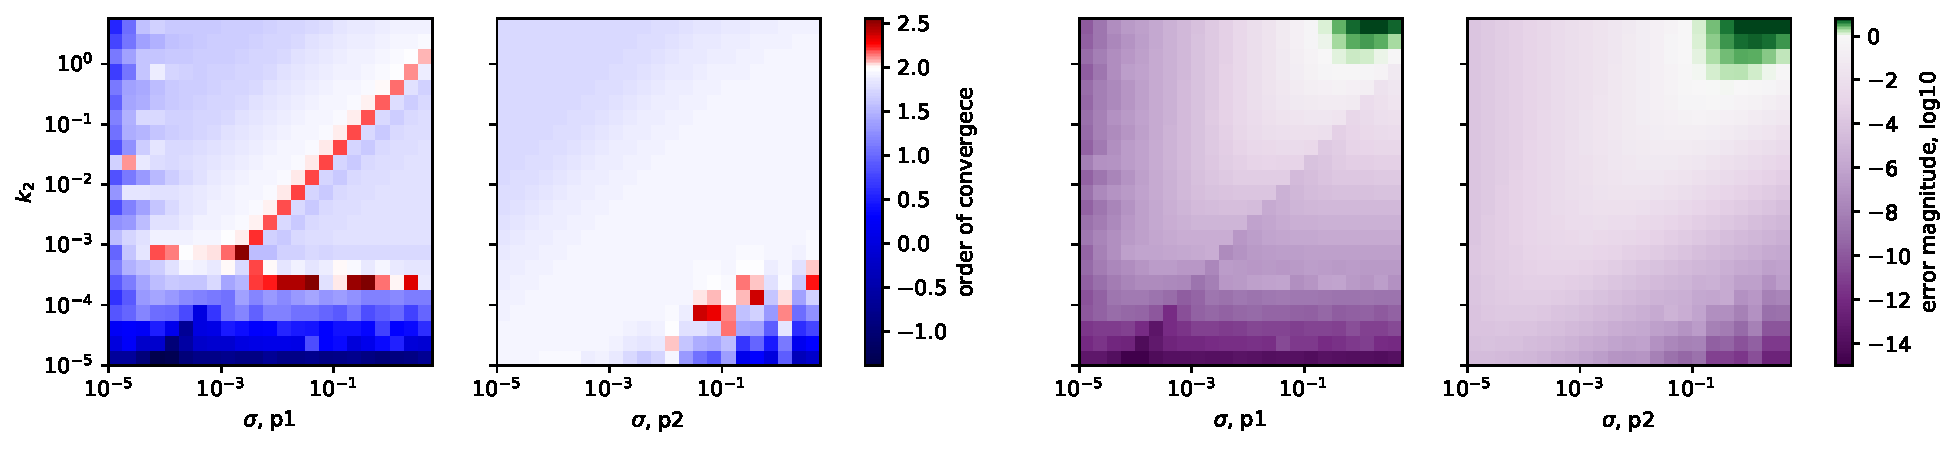
\includegraphics[width=\textwidth]{figs/continuous_conv_rate.pdf}
  % continuous_convergency.pdf: 0x0 pixel, 300dpi, 0.00x0.00 cm, bb=
  \caption{Convergence rate $p$ and absolute error exponent $c$ as a function of $k_2$ and $\sigma$. 
  {\it Left:} Order of convergence $p$ for $p_1$, $p_2$.
  {\it Right:} Absolute error exponent $c$ for $p_1$, $p_2$.}
  \label{fig:cont_rate}
\end{figure}





In this section, we aim to validate the derived analytical solutions by comparing them to a finite difference approximation, and investigate the convergence rate of the corresponding series as a function of the problem parameters. To achieve this, we have implemented the finite difference approximation of the system 
$(\ref{eq:Darcy_common} - \ref{eq:barrier_source})$, aproximating the first and second order derivatives directions using classical second order finite differences:
\begin{align*}
f'(x) &= \frac{-3 f(x) + 4f(x+h) - f(x+2h)}{2h} + O(h^2),\\
f''(x) &= \frac{-2 f(x) + f(x-h) + f(x+h)}{h^2} + O(h^2).
\end{align*}
The same grid step $h$ is assumed for both $x$ and $y$ direction
differences.

Figure \ref{fig:cont_solution} presents good match between the numerical solution ($h=0.01$) and the analytical solution truncated after $N=1000$ terms. 
Problem parameters were: $\sigma=20$, $k_1=10$, $k_2=1$, $P_2=10$, $P_1=5$.
Estimate for the sum reminder is $10^{-5}$. The magnitude of the error is of order $10^{-4}$. For the whole computationaly feasible range $h\in (0.1, 0.001)$ 
we have observed perfect second order convergence of the finite difference approximation. (TODO: if the error for N=1000 and h=0.001 can be decreased by more terms or by decrease of h, 
estimated error of analytical sol. is 1e-5, estimated FD error is 1e-6, so the truncation error should be dominant, but then we could not see ``prefect quardratic convergence'')

This is displayed at Figure \ref{fig:cont_rate} which contains results of a parametric study of the 
convergence rate as a function of parameters $k_1 \in [0.01, 0.1, 1, 10, 100]$ and $\sigma$ passing through the same set of values. The pressures $P_2=10$, $P_1=5$
and the conductivity $k_2=1$ are kept constant. For a fixed pair $k_1$, $\sigma$ we have estimated the rate of convergence by computing the finite difference solution for a sequence  
of mesh steps $0.1,\ 0.05,\ 0.025,\ 0.0125$. For every mesh step the $L^2$ errors $\epsilon_1$ and $\epsilon_2$ were approximated by the midpoint rule 
for $p_1$ and $p_2$ respectively. The order of convergence $p$ and the absolute error exponent $c$ were determined by the fit:
\[
        \log_2(\epsilon) \approx -c + p\log_2(h) 
\]

Clearly, the optimal second-order convergence or better is preserved for the majority of the parameter space. The drop to the linear convergence for combination 
of small $k_1$ and large $\sigma$ is due to extreme derivatives of $p_1$ close to the endpoints ${-1, 1}$. This behavior can not be resolved by the used regular grid.
Also, the absolute error exponent is well above $0$ so the error has a small magnitude. 

In the similar fashion we have tested the analytical solution to the barrier case. Shape of the solution and its match with the finite difference approximation 
is shown in Figure \ref{fig:barrier_solution}. The problem parameters were: $k_1=0.5$, $k_2^+=5$, $k_2^-=2$, $\sigma^+=20$, $\sigma^-=10$, $P_1=0$, 
$P_2^+=10$, $P_2^-=-10$, mesh step $h=0.01$. Notice the larger pressure gradient in lower part $\Omega^-$ with smaller conductivity $k_2^- = 2$, also the gap between 
$p_1(x)$ and $p_2(x, 0)$ is larger due to smaller value of $\sigma^- = 10$. 

The convergence rate for varying parameters is shown in Figure \ref{fig:barrier_rate}. In particular we have used $\sigma^+ = 3*\sqrt{\sigma}$, $\sigma^- = \sigma$
and $k_2^+ = k_2$, $k_2^- = \sqrt{k_2}$ with both $\sigma$ and $k_2$ iterating through the list $[0.01, 0.1, 1, 10, 100]$. Remaining parameters were fixed on 
following values: $k_1=1$, $P_2^+=10$, $P_2^-=-10$, $P_1=0$. Overall convergence rate is close to or beyond second order as in the previous case we see problems 
of the finite differences to resolve high gradient in $p_1$ for high $k_2$ and $\sigma$. Absolute error is also small for small $k_2$ which is natural since the 
solution (both $p_1$ and $p_2$) tends to be constant in $x$. 

\begin{figure}
  \label{fig:barrier_solution}
  \centering
  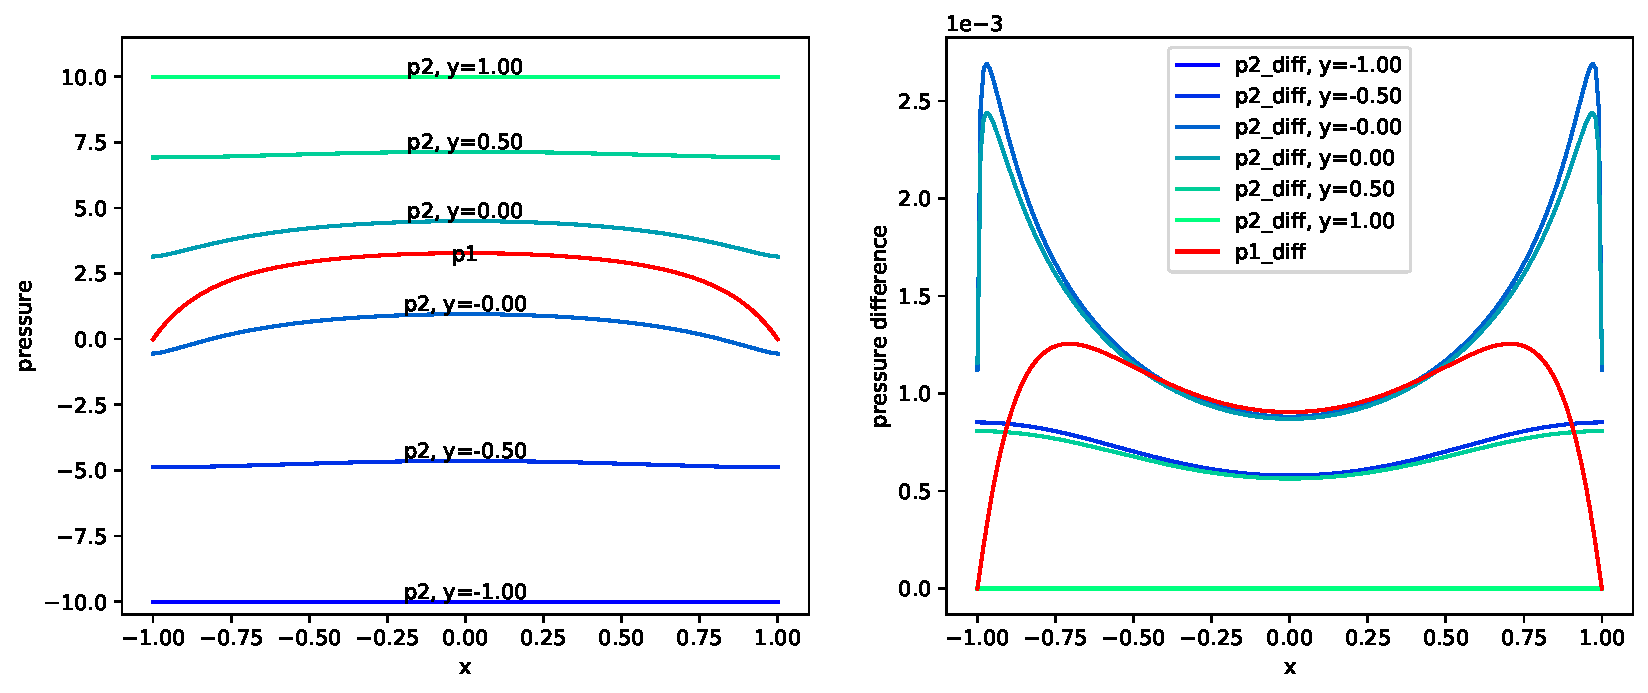
\includegraphics[width=\textwidth, keepaspectratio=true]{figs/barrier_solution.pdf}
  % continuous_convergency.pdf: 0x0 pixel, 300dpi, 0.00x0.00 cm, bb=
  \caption{Barrier fracture case.
  {\it Left:} Match between the analytical and the numerical solution. 
  {\it Right:} Difference of the analytical and the numerical solution.}
\end{figure}

\begin{figure}
  \label{fig:barrier_rate}
  \centering
  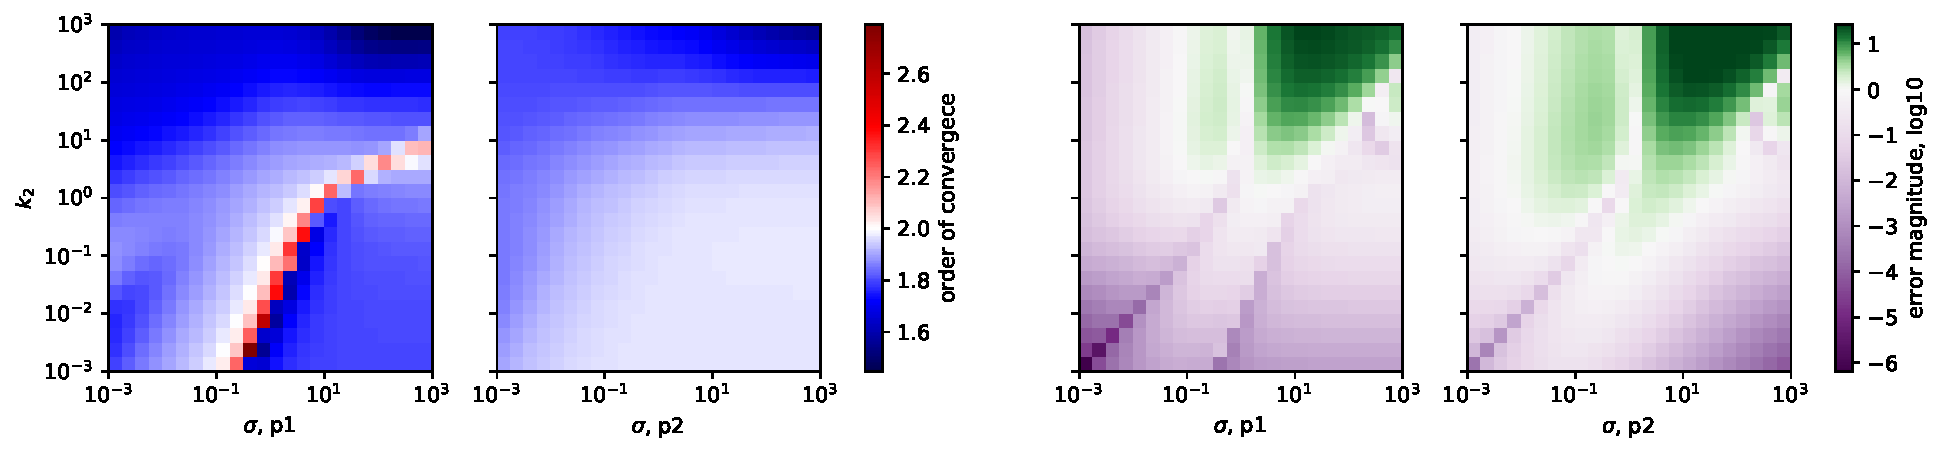
\includegraphics[width=\textwidth]{figs/barrier_conv_rate.pdf}
  % continuous_convergency.pdf: 0x0 pixel, 300dpi, 0.00x0.00 cm, bb=
  \caption{Convergence rate $p$ and absolute error exponent $c$ as a function of $k_2$ and $\sigma$. 
  {\it Left:} Order of convergence $p$ for $p_1$, $p_2$.
  {\it Right:} Absolute error exponent $c$ for $p_1$, $p_2$.}
\end{figure}


\section{Conclusion}
\label{sec:conclusion}
The analytical solution in a form of Fourier series has been derived for the symmetrical conductive fracture problem as well as for 
the general barrier fracture problem. The solution was modified for practical calculations and the convergence rate of the series was estimated theoretically and 
confirmed numerically. It was realized that summing $100$ terms provides precision about $10^{-6}$ which would be enough for most applications.
The adaptive summation can do even better. The analytical solution was successfully verified against a finite difference solution.  

The analytical solution is used as part of the test suit of the software Flow123d \cite{flow123d} to test various methods of coupling for both conforming 
and non-conforming mixed meshes.




\bibliography{analytical_fracture}



\end{document}

